In this thesis we will use \mocasin, a tool for the Model-of-Computation-based Analysis and Simulation of applications~\cite{menard_rapido21}.
This tool, formerly known as \texttt{pykpn}~\cite{menard_norcas16,goens_mcsoc18}, has been developed as part of a collaborative effort between multiple researchers at the Chair for Compiler Construction at TU Dresden.
While the tool itself is a joint contribution with the coauthors of~\cite{menard_rapido21}, many concepts introduced in this thesis have been implemented and tested using \mocasin.
As such, this section will explain the tool in-depth, to enable the description of the different implementations of contributions from this thesis implemented in \mocasin.

\begin{figure}[h]
	\centering
   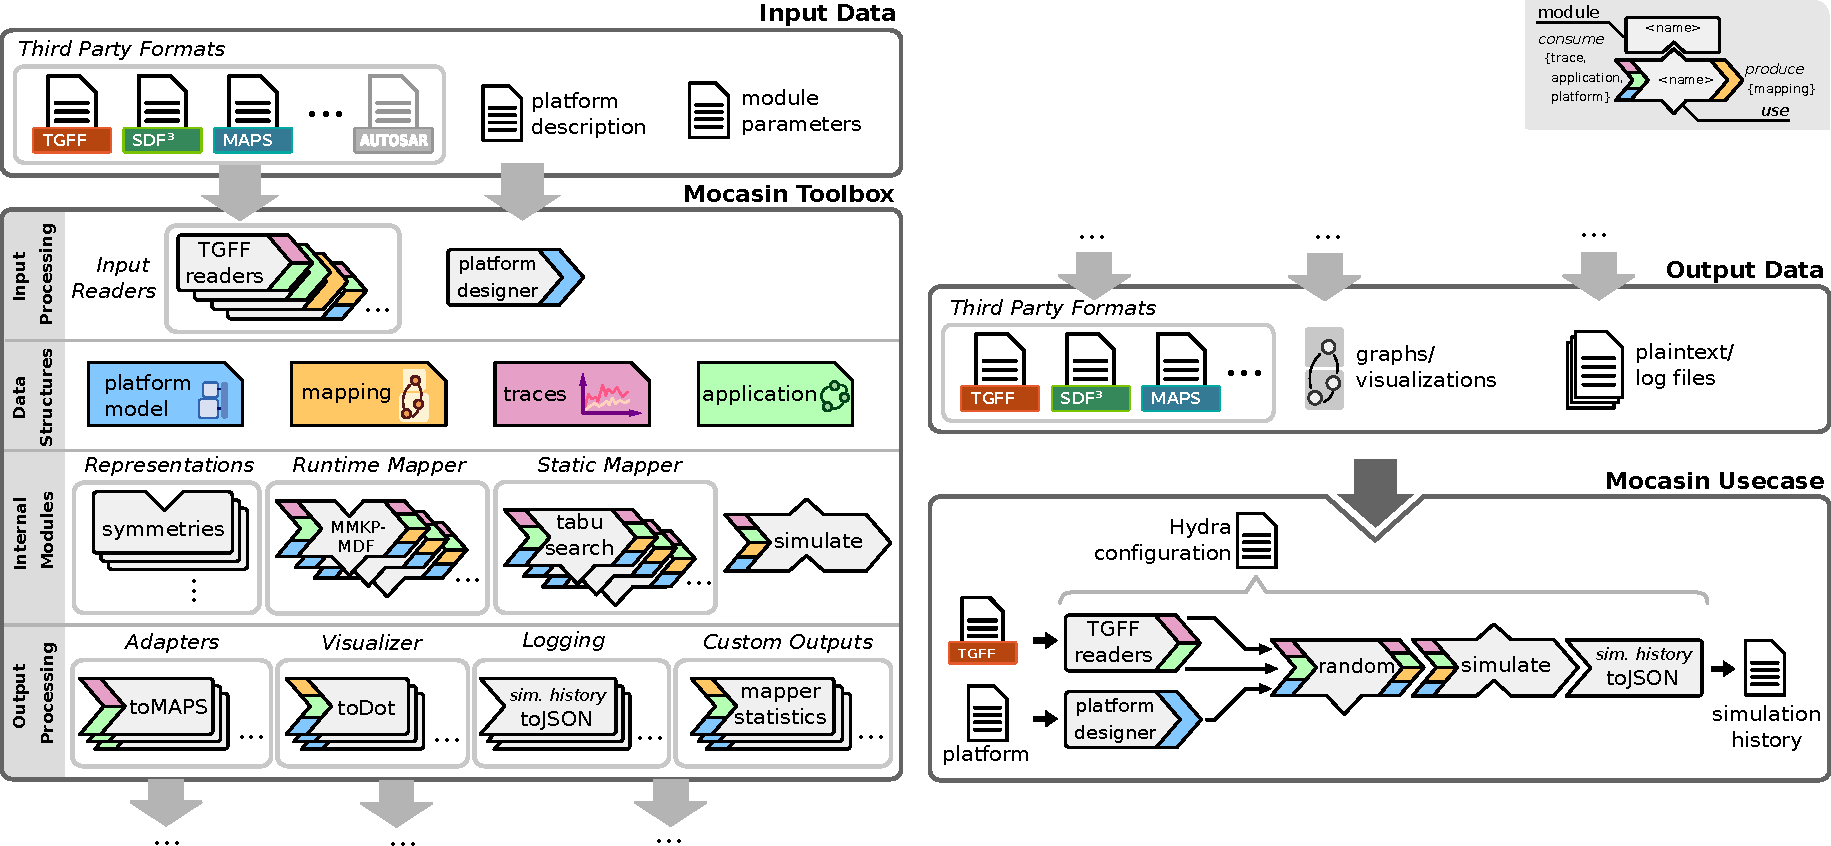
\includegraphics[width=0.95\textwidth]{figures/mocasin.pdf}
	\caption{The \mocasin architecture. Adapted from \cite{menard_rapido21} (Figure~2).}
	\label{fig:mocasin_arch}
\end{figure}


Figure~\ref{fig:mocasin_arch} depicts the basic flow of \mocasin.
It can be understood as a tool for rapid prototyping of prototyping tools.
Multiple dataflow \acp{MoC} are supported by \mocasin, like \ac{SDF} or task graphs.
These models, among others, can be seen as specializations of \ac{KPN}~\cite{lee1995dataflow} and will be discussed more in-depth in Chapter~\ref{chap:mocs}.
The \mocasin architecture is composed of multiple modules that can be combined to create a specific tool (e.g. for mapping or simulation). 

In general, simulating a KPN requires four inputs, as explained in Section~\ref{sec:mappings_background}: the KPN graph, a platform description, execution traces and a mapping.
\mocasin has data internal structures for these four inputs that reflect the models as explained in Sections~\ref{sec:kpn_basic,sec:traces,sec:arch_models,sec:mapping_problem}.
The tool boasts multiple readers to generate the internal data structures from established formats like \texttt{tgff}, \texttt{sdf3} or the \texttt{MAPS} formats. \index{tgff}\index{\acs*{\SDFFF}}
Instead of a concrete trace, \mocasin expects a trace generator, which can generate the trace on the fly: this is useful e.g. for non-deterministic models computation, but for KPNs the two are equivalent.
The \ac{KPN} trace generator, for example, simply reads the trace from a file.
A mapping, while required for simulation, does not need to be provided: it can be calculated in a design-space exploration.
This is not surprising, since a significant part of this thesis concerns itself with finding good mappings efficiently.

A central part of \mocasin is a discrete-event simulator~\cite{menard_norcas16} that uses the principles outlined above to simulate KPN applications based on their traces (as well as other models of computation).\index{discrete-event simulator}
We will not dwell on the design of the \texttt{simulate} module since it goes beyond the contribution and scope of this thesis.
In the following, we will describe some other central modules of \mocasin. 


\subsubsection{platform designer}

Many concepts developed in this thesis are aimed at emerging technologies and future hardware architectures.
To model these increasingly complex architectures, we aim at an abstract description of their topologies (cf. Section~\ref{sec:arch_models}).
As part of \mocasin, with the help of Felix Teweleitt, we designed a modeling infrastructure, in essence a small embedded domain-specific language, to describe hardware topologies.\index{platform designer}
This infrastructure is the \texttt{platform\_designer} module of \mocasin.

\begin{listing}
\begin{minted}[]{python}
designer = PlatformDesigner(self)
designer.setSchedulingPolicy('FIFO', 1000)
designer.newElement("Odroid-XU4")
# cluster 0 with l2 cache
designer.addPeClusterForProcessor("cluster_a7", processor_0, num_little)
# Add L1/L2 caches
designer.addCacheForPEs("cluster_a7", 1, 0, 8.0, float('inf'),
                        frequencyDomain=1400000000.0, name='L1_A7')
designer.addCommunicationResource("L2_A7", ["cluster_a7"], 250, 250,
                                  float('inf'), float('inf'),
                                  frequencyDomain=1400000000.0)
# cluster 1, with l2 cache
designer.addPeClusterForProcessor("cluster_a15", processor_1, num_big)
# Add L1/L2 caches
designer.addCacheForPEs("cluster_a15", 1, 4, 8.0, 8.0,
                        frequencyDomain=2000000000.0, name='L1_A15')
designer.addCommunicationResource("L2_A15", ["cluster_a15"], 250, 250,
                                  float('inf'), float('inf'),
                                  frequencyDomain=2000000000.0)
# RAM connecting all clusters
designer.addCommunicationResource("DRAM", ["cluster_a7", "cluster_a15"],
                                  120, 120, 8.0, 8.0,
                                  frequencyDomain=933000000.0)
designer.finishElement()
\end{minted}
\caption{The Odroid-XU4 Platform with the Platform Designer}
\label{listing:designer_odroid}
\end{listing}

Listing~\ref{listing:designer_odroid} shows an example of our \texttt{platform\_designer}.
The code in this listing describes the topology of the Odroid XU4 (see Figure~\ref{fig:odroid}). 
The main principle innovation behind the \texttt{platform\_designer} is that it works with a stack of clusters.
The functions \texttt{newElement()} and \texttt{finishElement()} can be nested to describe the topology in a hierarchical fashion.\index{hierarchical topologies}
Between these functions, the \ac{API} allows us to describe heterogeneous cores and different levels of interconnects with different properties, like their frequency.

\subsubsection{mappers}

The mapping problem (cf. Section~\ref{sec:mapping_problem}) plays an important role in this thesis.
While we do propose some mapping heuristics for special contexts, many methods in this thesis are orthogonal to the mapping heuristics.
As part of this thesis we have implemented multiple mapping algorithms from literature in \mocasin.
These can be found in the \texttt{mapper} module. 
The heursitics included are the \ac{GBM} heuristic~\cite{castrillon_dac12} and a static variant of the Linux \ac{CFS}.
We also have some meta-heuristics, which include a random walk, simulated annealing~\cite{simulated_annealig}, tabu search~\cite{tabu_search} and genetic algorithms~\cite{erbas2006multiobjective,goens_mcsoc16}. 

\subsubsection{configuration}

\mocasin is designed to be a tool for tool development.
As such, one of its main goals is to enable building different scenarios for different contexts, like static mapping of \ac{KPN} applications or hybrid execution of dynamic \ac{LTE} loads~\cite{menard_rapido21}.
We use the Hydra~\ref{yadan2019-hydra} framework to configure \mocasin and construct different scenarios as different tools.\index{Hydra}
Figure~\ref{fig:mocasin_arch} depicts this to the right, for an example simulating \ac{tgff} applications with random mappings and storing the execution history in a \texttt{JSON} file.
This configuration philosophy allows us to work in a modular fashion, with the modules as depicted in the \mocasin toolbox in the figure.
This allows us to implement different contributions of this thesis as \mocasin modules.

\subsubsection{contributions}

Many concepts that are central contributions of this thesis are implemented in \mocasin. 
This is done as modules, using the \mocasin toolbox infrastructure. 
Figure~\ref{fig:mocasin_kpn_simulation} shows a family of \mocasin flows for mapping and simulating KPN or \ac{tgff} applications.
Different contributions of this thesis and the corresponding references are described in the figure and marked as such (with light-green coloring).

\begin{figure}[h]
	\centering
   \resizebox{0.95\textwidth}{!}{% Define block styles
\tikzstyle{mio} = [rectangle, rounded corners, draw, fill=green!20, %legend: possible "IP leak"
    text width=7em, text centered, minimum height=4em]
\tikzstyle{block} = [rectangle, draw, fill=blue!20, 
    text width=7em, text centered, rounded corners, minimum height=4em]
\tikzstyle{required} = [draw, ->]
\tikzstyle{possible} = [draw, dashed, ->]
\tikzstyle{interaction} = [thick, <->, draw, color=red!70]
\tikzstyle{data} = [rectangle, rounded corners, draw, fill=teal!20, text width=7em, text centered,  minimum height=4em]

\begin{tikzpicture}[node distance = 4em]
    % inputs/readers
    \node [block ] (tgff) {tgff readers};
    \node [block, below=of tgff ] (sdf3) {sdf$^3$ readers};
    \node [block, below=of sdf3] (slx) {SLX readers};

    %data
    \node [data, right=of tgff] (traces) {traces};
    \node [data, below=of traces] (app) {application (e.g. KPN)};
    \node [data, below=of app] (mapping) {mapping};
    \node [data, below=of mapping] (platform) {platform model};

    \node [block, left=of platform] (platformdes) {platform designer};

    %modules
    \node [block, right=of mapping] (mappers) {mappers};
    \node [block, right=of app] (simulate) {simulate};
    \node [mio, above=of simulate] (tetris) {runtime managers (Section~\ref{sec:tetris}) };
    \node [mio, right=of mappers] (logic) {logic language manager (Section~\ref{sec:logic_language})};
    \node [mio, below=of mappers] (representations) {representations (Chapter~\ref{chap:mapping_structures})};
    \node [mio, above=of logic, align=center] (dc) {design centering \\ (Section~\ref{sec:design_centering})};


    %edges
    \path [possible] (slx) -- (traces);
    \path [possible] (slx) -- (app);
    \path [possible] (slx) -- (platform);
    \path [possible] (slx) -- (mapping);

    \path [possible] (tgff) -- (traces);
    \path [possible] (tgff) -- (app);
    \path [possible] (sdf3) -- (traces);
    \path [possible] (sdf3) -- (app);

    \path [possible] (platformdes) -- (platform);

    \path [required] (traces) -- (mappers);
    \path [required] (app) -- (mappers);
    \path [required] (platform) -- (mappers);
    \path [required] (mappers) -- (mapping);



    \path [required] (traces) -- (simulate);
    \path [required] (app) -- (simulate);
    \path [required] (platform) -- (simulate);
    \path [required] (mapping) -- (simulate);

    %interactions
    \path [interaction] (mappers) -- (logic);
    \path [interaction] (mappers) -- (representations);
    \path [interaction] (simulate) -- (tetris);
    \path [interaction] (simulate) -- (mappers);
    \path [interaction] (simulate) -- (dc);

    \matrix [draw=black,fill=gray!10,above=13em of traces.north west, anchor=north west] {
      \node[data, rounded corners=0, text width=1em, minimum height=1em] {}; & \node[] {data structure};\\
      \node[block, rounded corners=0, text width=1em, minimum height=1em] {}; & \node[] {module};\\
      \node[mio, rounded corners=0, text width=1em, minimum height=1em] {}; & \node[] {module with contributions from this thesis};\\
      \draw[possible] (0,-0.2) -- (0.4,-0.2); & \node[] {optional input data};\\
      \draw[required] (0,-0.2) -- (0.4,-0.2); & \node[] {internal data depencency};\\
      \draw[interaction] (0,-0.2) -- (0.4,-0.2); & \node[] {interaction between modules};\\
      % \node[fill=black,draw,circle,inner sep=2pt,outer sep=0pt] (m) at (0,0){};
      % \draw (m) -- +(0,0.4); & \node[legendtext]{Mandatory}; & 
 %   \filldraw[fill=white,draw=black] (0,0.2) -- ++(225:0.2) arc[start angle=225,end angle=315,radius=0.2]; 
 % \draw (0,0.2) ++(225:0.5) -- (0,0.2) -- ++(315:0.5);& \node[legendtext]{Alternative}; \\
 %  \node[fill=white,draw=black,circle,inner sep=2pt,outer sep=0pt] (o) at (0,0){}; \draw (m) -- +(0,0.4); & \node[legendtext]{Optional}; & 
 %  \draw (0,0.2) ++(225:0.5) -- (0,0.2) -- ++(315:0.5);
 %  \filldraw[black] (0,0.2) -- ++(225:0.2) arc[start angle=225,end angle=315,radius=0.2]; & \node[legendtext]{Or}; 
\\
};
\end{tikzpicture}
}
	\caption{Mapping and simulating KPN Applications in \mocasin.}
	\label{fig:mocasin_kpn_simulation}
\end{figure}